\section{Optimizations}
\label{sec:optimizations}

In implementing \tritonsort, we learned that several non-obvious optimizations
were necessary to meet our desired disk bandwidth goals.  Here, we present the
key takeaways from our experience.

\subsection{Network}
\label{sec:fastnetwork}

\begin{figure}
  \centering
  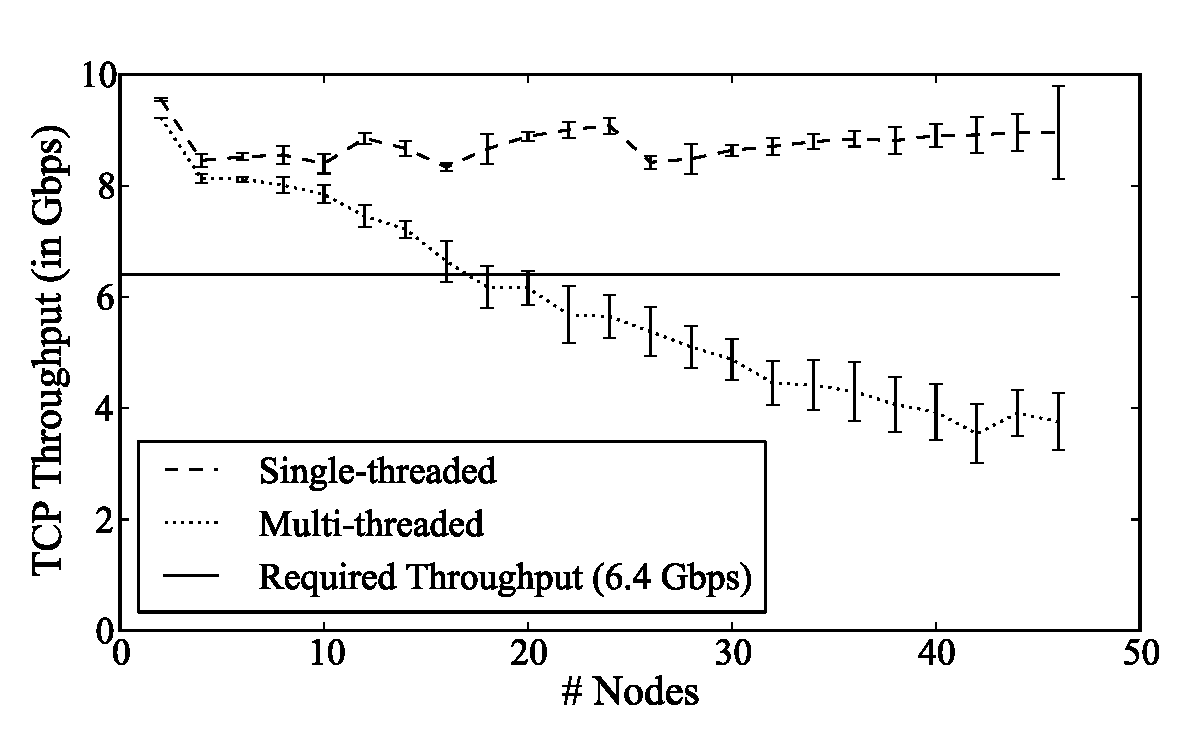
\includegraphics[width=\columnwidth]{tritonsort/graphs/netscalability.pdf}

\caption{Comparing the scalability of single-threaded and
  multi-threaded \receiver implementations.}
  \label{fig:net_scalability}
\end{figure}

For \tritonsort to operate at the aggregate sequential streaming bandwidth of
all of its disks, the network must be able to sustain the read throughput of
eight disks while data is being shuffled among nodes in the first phase.  Since
the 7.2k-RPM disks we use deliver at most 100 MBps of sequential read
throughput (Table~\ref{tab:resourcesummary}), the network must be able to
sustain 6.4 Gbps of all-pairs bandwidth, irrespective of the number of nodes in
the cluster.

It is well-known that sustaining high-bandwidth flows in datacenter networks,
especially all-to-all patterns, is a significant challenge.  Reasons for this
include commodity datacenter network hardware, incast, queue buildup, and
buffer pressure\cite{dctcp}.  Since we could not employ a strategy like that
presented in \cite{dctcp} to provide fair but high bandwidth flow rates among
the senders, we chose instead to artificially rate limit each flow at the
\sender stage to its calculated fair share by forcing the sockets to be receive
window limited.  This works for \tritonsort because 1) each machine sends and
receives at approximately the same rate, 2) all the nodes share the same RTT
since they are interconnected by a single switch, and 3) our switch
does not impose an oversubscription factor.  In this case, each \sender should
ideally send at a rate of $(6.4 / N)$ Gbps, or 123 Mbps with a cluster of 52
nodes.  Given that our network offers approximately $100 \mu{}sec$ RTTs, a
receiver window size of $8-16$ KB ensures that the flows will not impose queue
buildup or buffer pressure on other flows.

Initially, we chose a straightforward multi-threaded design for the \sender and
\receiver stages in which there were $N$ \senders and $N$ \receivers, one for
each \tritonsort node.  In this design, each \sender issues blocking
\textit{send()} calls on a \nodebuffer until it is sent.  Likewise, on the
destination node, each \receiver repeatedly issues blocking \textit{recv()}
calls until a \nodebuffer has been received.  Because the number of CPU
hyperthreads on each of our nodes is typically much smaller than $2N$, we
pinned all \senders' threads to a single hyperthread and all \receivers'
threads to a single separate hyperthread.

Figure~\ref{fig:net_scalability} shows that this multi-threaded approach does
not scale well with the number of nodes, dropping below 4 Gbps at scale.  This
poor performance is due to thread scheduling overheads at the end hosts.  16 KB
TCP receive buffers fill up much faster than connections that are not
window-limited.  At the rate of 123 MBps, a 16 KB buffer will fill up in just
over 1 ms, causing the \sender to stop sending.  Thus, the \receiver stage must
clear out each of its buffers at that rate.  Since there are 52 such buffers, a
\receiver must visit and clear a receive buffer in just over 20 $\mu$s.  A
\receiver worker thread cannot drain the socket, block, go to sleep, and get
woken up again fast enough to service buffers at this rate.

To circumvent this problem we implemented a single-threaded, non-blocking
receiver that scans through each socket in round-robin order, copying out any
available data and storing it in a \nodebuffer during each pass through the
array of open sockets.  This implementation is able to clear each socket's
receiver buffer faster than the arrival rate of incoming data.
Figure~\ref{fig:net_scalability} shows that this design scales well as the
cluster grows.

\subsection{Minimizing Disk Seeks}
\label{sec:diskseeks}

\begin{figure}
  \centering
  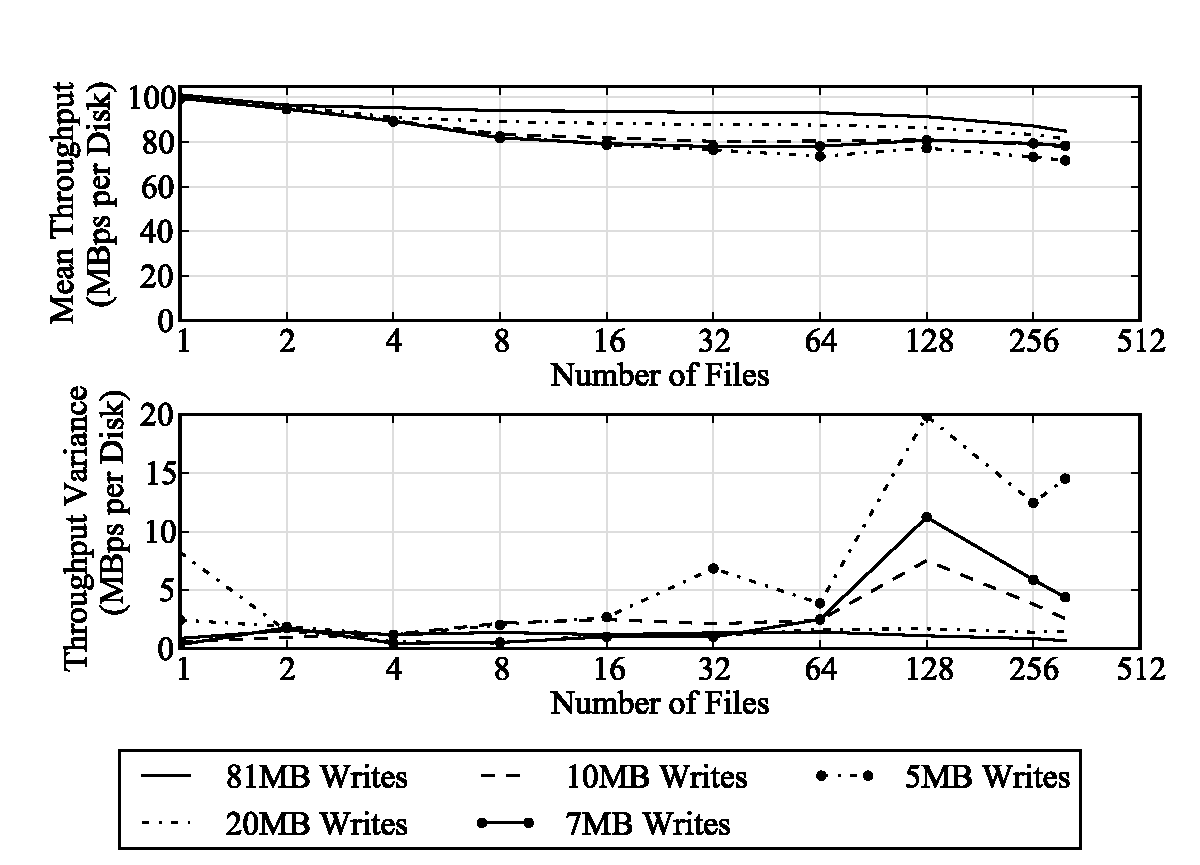
\includegraphics[width=\columnwidth]{tritonsort/graphs/write_scalability_throughput_receiverbench}
  \caption{\label{fig:micro_write_bw}Microbenchmark indicating the ideal disk throughput as a function of
           write size.}
\end{figure}

Key to making the \tritonsort pipeline efficient is minimizing the total amount
of time spent performing disk seeks, both while writing data in phase one, and
while reading that data in phase two.  As individual write sizes get smaller,
write throughput drops, since the disk must occasionally seek between
individual write operations.  Figure~\ref{fig:micro_write_bw} shows disk write
throughput measured by a synthetic workload generator writing to a configurable
set of files with different write sizes.  Ideally, the \writer would receive
\writerbuffers large enough that it can write them out at close to the
sequential rate of the disk.  However, the amount of available memory limits
\tritonsort's write sizes.  Since the record space is uniformly distributed
across the logical disks, the \ldts will fill its \ldbuffer{}s at approximately
a uniform rate.  Buffering 80 MB worth of records for a given logical disk
before writing to disk would cause the buffers associated with all of the other
logical disks to become approximately as full.  This would mandate
significantly higher memory requirements than what is available in our hardware
architecture.  Hence, the \ldts stage must emit smaller \writerbuffer{}s, and
it must interleave writes to different logical disks.

\subsection{The Importance of File Layout}

The physical layout of individual logical disk files plays a strong role in
trading off performance between the phase one \writer and the phase two
\reader.  One strategy is to append to the logical disk files in a
log-structured manner, in which a \writerbuffer for one logical disk is
immediately appended after the \writerbuffer for a different logical disk.
This is possible if the logical disks' blocks are allocated on demand.  It has
the advantage of making the phase one \writer highly performant, since it
minimizes seeks and leads to near-sequential write performance.  On the other
hand, when a phase two \reader begins reading a particular logical disk, the
underlying physical disk will need to seek frequently to read each of the
\writerbuffer{}s making up the logical disk.

An alternative approach is to greedily allocate all of the blocks for each of
the logical disks at start time, ensuring that all of a logical disk's blocks
are physically contiguous on the underlying disk.  This can be accomplished
with the \texttt{fallocate()} system call, which provides a hint to the file
system to pre-allocate blocks.  In this scheme, interleaved writes of
\writerbuffer{}s for different logical disks will require seeking, since two
subsequent writes to different logical disks will need to write to different
regions on the disk.  However, in phase two, the \reader will be able to
sequentially read an entire logical disk with minimal seeking. We also use
\texttt{fallocate()} on input and output files so that phase one \readers and
phase two \writers seek as little as possible.

The location of output files on the output disks also has a dramatic effect on
phase two's performance.  If we do not delete the input files before starting
phase two, the output files are allocated space on the interior cylinders of
the disk.  When evaluating phase two's performance on a 100 TB sort, we found
that we could write to the interior cylinders of the disk at an average rate of
~64 MBps.  When we deleted the input files before phase two began, ensuring that
the output files would be written to the exterior cylinders of the disk, this
rate jumped to 84 MBps.  For the evaluations in Section~\ref{sec:evaluation}, we
delete the input files before starting phase two.  For reference, the fastest
we have been able to write to the disks in microbenchmark
has been approximately 90 MBps.

\subsection{CPU Scheduling}

Modern operating systems support a wide variety of static and dynamic CPU
scheduling approaches, and there has been considerable research into scheduling
disciplines for data processing systems.  We put a significant amount of effort
into isolating stages from one another by setting the processor affinities of
worker threads explicitly, but we eventually discovered that using the default
Linux scheduler results in a steady-state performance that is only about 5\%
worse than any custom scheduling policy we devised.  In our evaluation, we use
our custom scheduling policy unless otherwise specified.

\subsection{Pipeline Demand Feedback}
\label{sec:tritonsort-disk-scheduler}

Initially, \tritonsort was entirely ``push''-based, meaning that a worker only
processed work when it was pushed to it from a preceding stage.  While simple
to design, certain stages perform sub-optimally when they are unable to send
feedback back in the pipeline as to what work they are capable of doing.  For
example, the throughput of the \writer stage in phase one is limited by the
latency of writes to the intermediate disks, which is governed by the sizes of
\writerbuffer{}s sent to it as well as the physical layout of logical disks
(due to the effects of seek and rotational delay).  In its \naive
implementation, the \ldts sends work to the \writer stage based on which of its
\ldbuffer lists is longest with no regard to how lightly or heavily loaded the
\writers themselves are.  This can result in an imbalance of work across
\writers, with some \writers idle and others struggling to process a long queue
of work.  This imbalance can destabilize the whole pipeline and lower total
throughput.

To address this problem, we must effectively communicate information about the
sizes of \writers' work queues to upstream stages.  We do this by creating a
pool of \emph{write tokens}. Every write token is assigned a single ``parent''
\writer. We assign parent \writers in round-robin order to tokens as the tokens
are created and create a number of tokens equal to the number of
\writerbuffers.
When the \ldts has buffered enough \ldbuffers so that one or more of its logical
disks is above the minimum write threshold (5MB), the \ldts will query the
write token pool, passing it a set of \writers for which it has enough data.
If a write token is available for one of the specified \writers in the set, the
pool will return that token; otherwise, it will signal that no tokens are
available.  The \ldts is required to pass a token for the target \writer along
with its \ldbuffer list to the next stage, This simple mechanism prevents any
\writer's work queue from growing longer than its ``fair share'' of the
available \writerbuffers and provides reverse feedback in the pipeline without
adding any new architectural features.

\subsection{System Call Behavior}

In the construction of any large system, there are always idiosyncrasies in
performance that must be identified and corrected.  For example, we noticed
that the sizes of arguments to Linux \texttt{write()} system calls had a
dramatic impact on their latency; issuing many small writes per buffer often
yielded more performance than issuing a single large write.  One would imagine
that providing more information about the application's intended behavior to
the operating system would result in better management of underlying resources
and latency but in this case, the opposite seems to be true.  While we are
still unsure of the cause of this behavior, it illustrates that the performance
characteristics of operating system services can be unpredictable and
counter-intuitive.

%LocalWords: incast RTT oversubscription Mbps RTTs recv hyperthreads epoll
%LocalWords: Microbenchmark record records performant pre microbenchmark
